\documentclass[12pt]{article}

%Graphic packages
\usepackage{graphicx}
\usepackage{subcaption}
\graphicspath{ {../Images} }

%References libraries
\usepackage{hyperref}
\usepackage[super]{natbib}

%Format
\usepackage{placeins}
\usepackage{geometry}
\geometry{includeheadfoot,a4paper, textwidth=0.87\paperwidth, textheight=0.9\paperheight, headsep =30pt}
\usepackage[onehalfspacing]{setspace}
\usepackage{fancyhdr}
\pagestyle{fancy}
\renewcommand{\headrulewidth}{1.5pt}
\lhead{
\includegraphics[scale=0.05]{SB.png}}
\rhead{
\includegraphics[scale=0.1]{IDL.png}}
\chead{Docking methods}
\usepackage{multicol}

%Chemistry packages
\usepackage{mol2chemfig}
\usepackage{chemfig}
\usepackage{caption}
\usepackage{chemmacros}

%Math and table packages
\usepackage{amssymb}
\usepackage{multicol}
\usepackage{multirow}
\usepackage{booktabs}
\usepackage[para,online,flushleft]{threeparttable}
\usepackage{float}

%
%\usepackage{lmodern}
%\usepackage[T1]{fontenc}
%\usepackage{anyfontsize}
%\newcommand\chemsize{\fontsize{5pt}{6pt}\selectfont}

\begin{document}
	\title {Docking Methods}
	\date{iGEM Design League 2022}
	\author{Synthetic Biobots\\Gerardo Cendejas Mendoza}
	
	\maketitle

	\begin{center}
		
\includegraphics[scale=0.4]{SB.png}
	\end{center}
	\newpage
	
	\phantomsection
	\addcontentsline{toc}{section}{Introduction}
	\section*{Introduction}
	
	In this document is shown the docking methodology followed by the team  Synthetic Biobots during the iGEM Design League 2022 season. Molecular docking is a process to couple proteins with their ligands; for this project molecular docking was performed in order to support the decision of using the proteins that were selected as part of the biosynthetic pathway of piperamide. The different steps necessary for its production are shown in the \hyperlink{pathway}{figure} shown in the next page; in this figure all the steps required are marked with a number, this number is an identifier for the enzyme required to perform that step.\\
	
	From all the enzymes used in the pathway, only 8 require a docking step for different reasons, these reasons can be that it is an enzyme that has not been isolated and even though a previous annotation step indicates it performs that reaction, molecular docking can provide better support for their selection and activity. Another reason to perform molecular docking is when the protein is known and has been isolated but we are using a molecule that is not the original ligand of the protein, in this case molecular docking can help to elucidate if the protein is capable of performing the reaction with a molecule with similar structure to its original ligand. The enzymes that are subject of molecular docking and the genes that code for these enzymes and will be studied are: 1 (Pn8.2617), 2 (Pn2.84), 4 (Pn1.1317), 5 (Pn3.4770, Pn7.1626), 6 (Pn16.1237, Pn16.1198), 8 (Pn4.3222), 9 (Pn2.2377) and 10 (\href{https://www.rcsb.org/structure/2CWH}{2cwh}).\\
	
	For each of these genes it was performed a differential exon usage analysis between four different \textit{Piper nigrum} tissues: fruit at 20 days stage, fruit at 40 days stage, leaf and panicle. This analysis can help us to visualize the expression level for each exon of the genes, this information allows us to select the exons of the gene to include in the modeling and in the following steps. This analysis was performed by using the Bioconductor library ``DEXSeq'', to access the code used for this methodology please visit the GitHub repository of the team for iGEM Design League 2022 season, the \href{https://github.com/GerardoCMM/Synthetic-Biobots-IGEM-DL-2022/tree/main/Exon_usage}{Exon\_usage} directory. \cite{bioconductor,dexseq,dexseq_2}\ \ The STAR ultrafast universal RNA-seq aligner on the Galaxy project platform mapped the RNA-seq reads to the reference genome of \textit{Piper nigrum} prior to the differential exon usage analysis. \cite{genome,star,galaxy}\ \ Only results of relevance for the modeling and docking methods are shown in this document.
	
	
	
	
	\FloatBarrier
	\begin{figure}[h]
		\centering
		\hypertarget{pathway}{}
		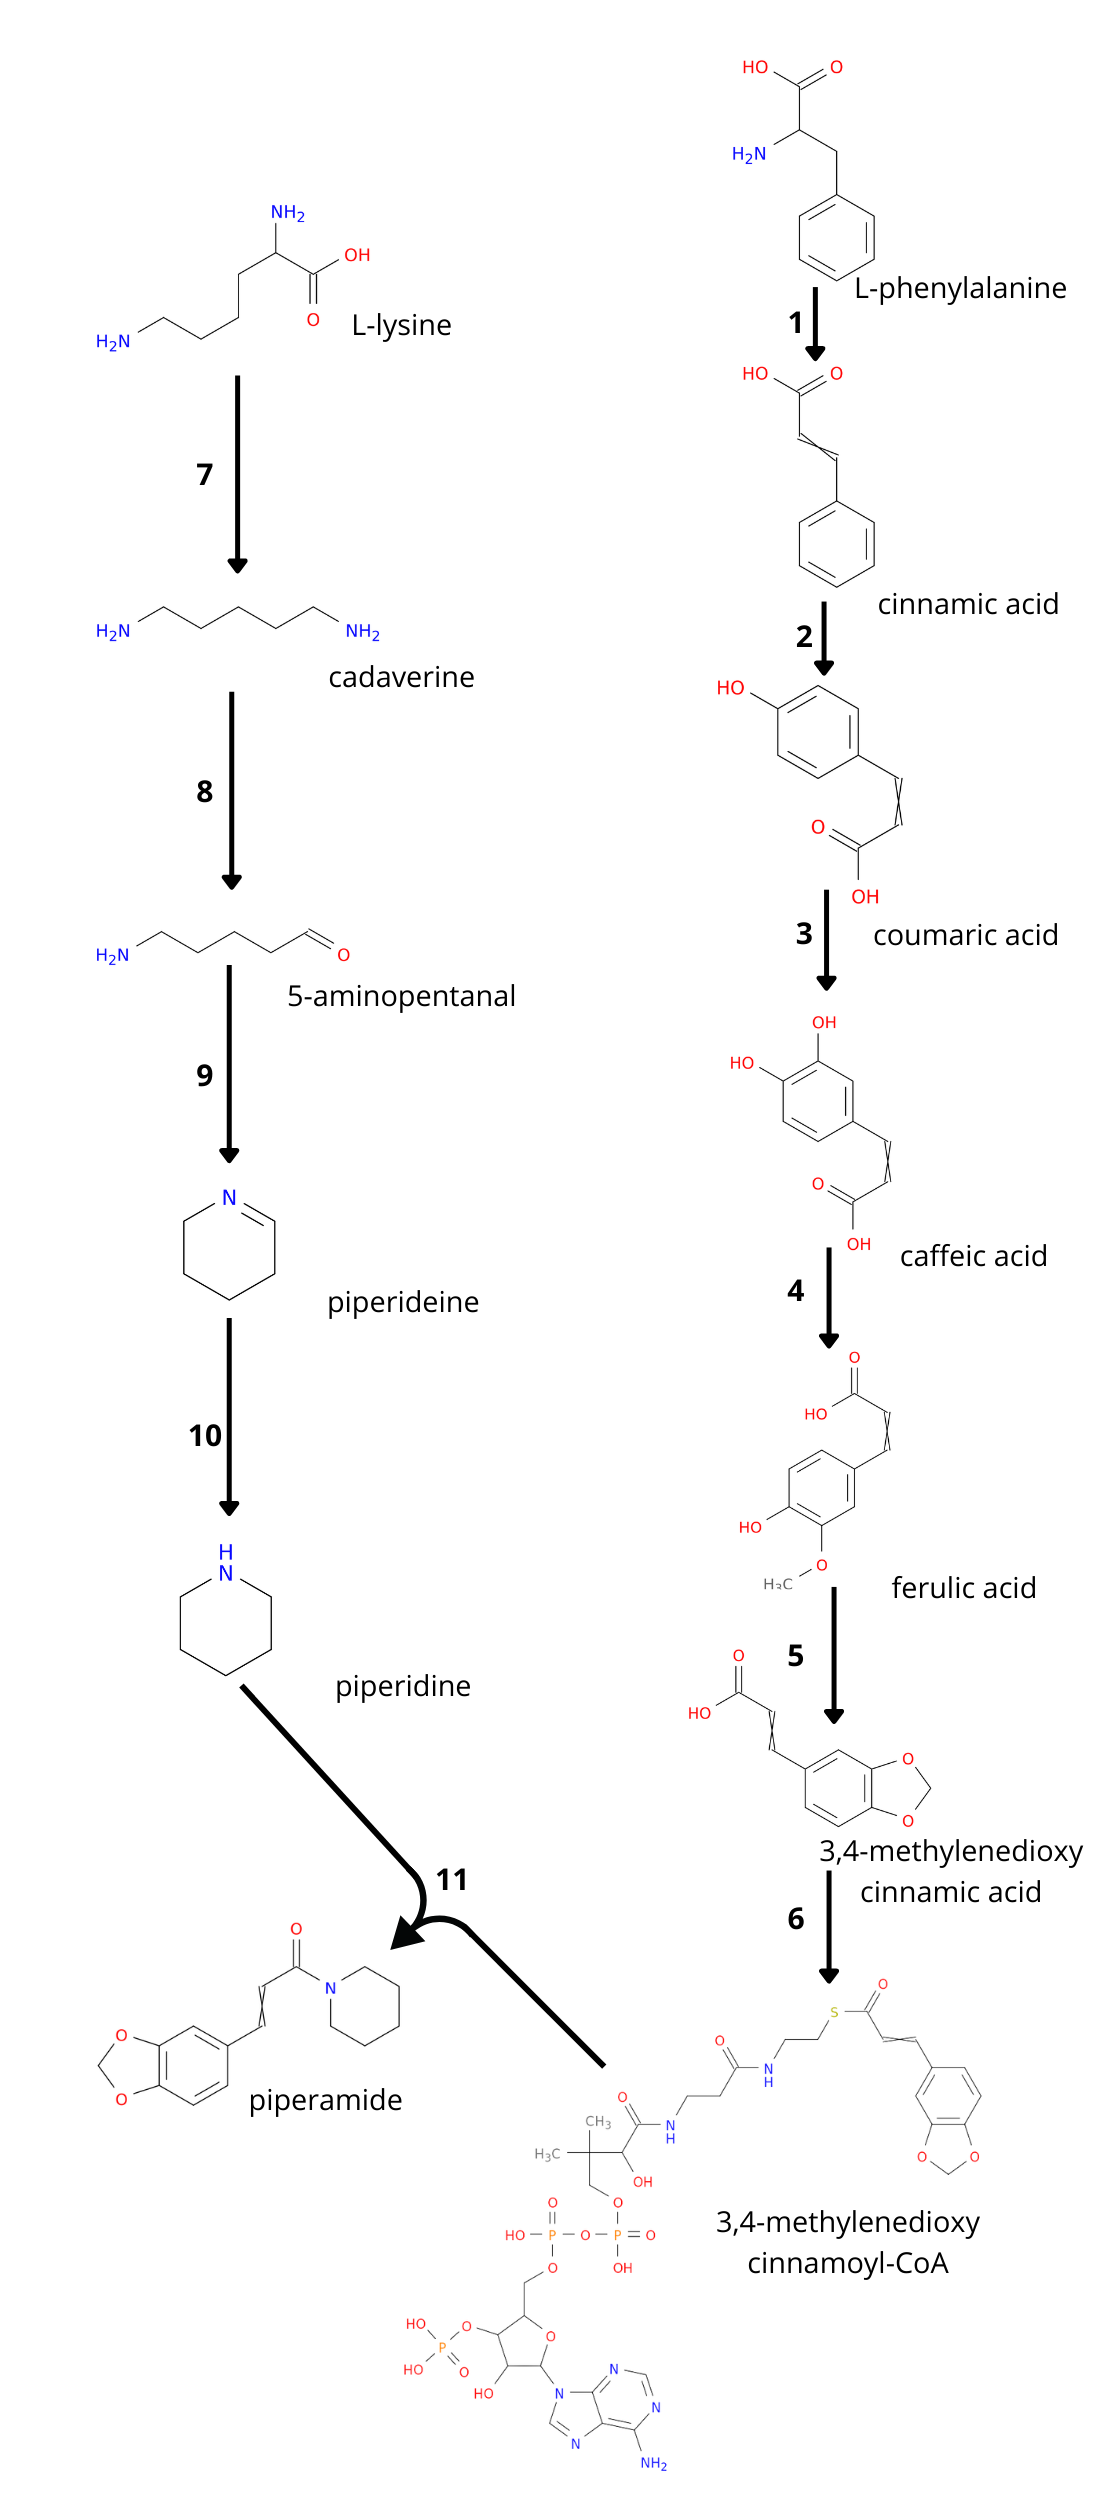
\includegraphics[scale=0.35]{Pathway2.png}
		\caption*{Biosynthetic pathway of piperamide.}
		
	\end{figure}
	\FloatBarrier
	
	
	\section{Docking}
	
	\subsection{Pn8.2617}
	
	The first reaction in the biosynthetic pathway of piperamide is performed by the enzyme phenylalanine ammonia-lyase, which is part of the phenylpropanoid biosynthesis pathway and catalyzes the reaction shown in Eq. \ref{eq1}. The gene Pn8.2617 was selected as the best candidate for enzyme 1, this selection was based on the fact that it obtained the highest score (1170.9) over the threshold (524.93) for KEGG Orthology ID K10775, with E-value $\approxeq 0$ . This annotation was made with KofamKOALA. \cite{kofamkoala} With the exon usage analysis no relevant results were found.
	
	
	\begin{equation}
		\schemestart
		 \label{eq1}
		\chemname{\footnotesize\chemfig{O=[:90](-[:30,,,1]OH)-[:150](-[:90,,,1]NH_2)-[:210]-[:150]-[:90]%
-[:150]-[:210](-[:330,,,,draw=none]\mcfcringle{1.3})-[:270]-[:330](-[:30])}
}{Phenylalanine}\arrow{->[\footnotesize 1]}\chemname{\footnotesize\chemfig{O=[:90](-[:30,,,1]OH)-[:150]-[:210,,,,drh]-[:150]-[:90]-[:150]%
-[:210](-[:330,,,,draw=none]\mcfcringle{1.3})-[:270]-[:330](-[:30])}
}{Cinnamic acid}
		\arrow{0}[,0]+
		\chemname{\footnotesize\chemfig{NH_3}}{Ammonia}
		\schemestop
	\end{equation}\\
	
	The gene contains two exons that were considered when modeling the three-dimensional structure of the protein. The structure modeling was made by using an homology based methodology ``SWISS-MODEL''. \cite{swiss,quaternary_swiss} This methodology is template based, in this case the template selected was a phenylalanine ammonia-lyase from \textit{Petroselinum crispum} with PDB ID: \href{https://www.rcsb.org/structure/1w27}{1w27}; this protein has a 79.97\% sequence identity to our query protein Pn8.2617 which make it an appropiate template. The template was found with HHblits, a protein sequence searching algorithm that uses hmm-hmm alignment. \cite{hhblits} The model (Fig. \ref{fig1_1}) is found in a homo-tetrameric state, as the template is; it has a GMQE value of 0.84 and a QMEANDisCo Global value of 0.81 ± 0.05 (Fig. \ref{fig1_2}). The QMEANDisCo value is a composite score value for single model quality estimation, this value is a function of underlying single model scores employing statistical potentials of mean force and a distance constraint based on the known structure of homologous proteins. QMEANDisCo value is calculated for every residue of the protein and the QMEANDisCo Global value is the average of these per residue scores, which aims to be a good approximation of the global overall quality of the model. \cite{qmeandisco_swiss}

	
	\FloatBarrier
	\begin{figure}[H]
		\centering
		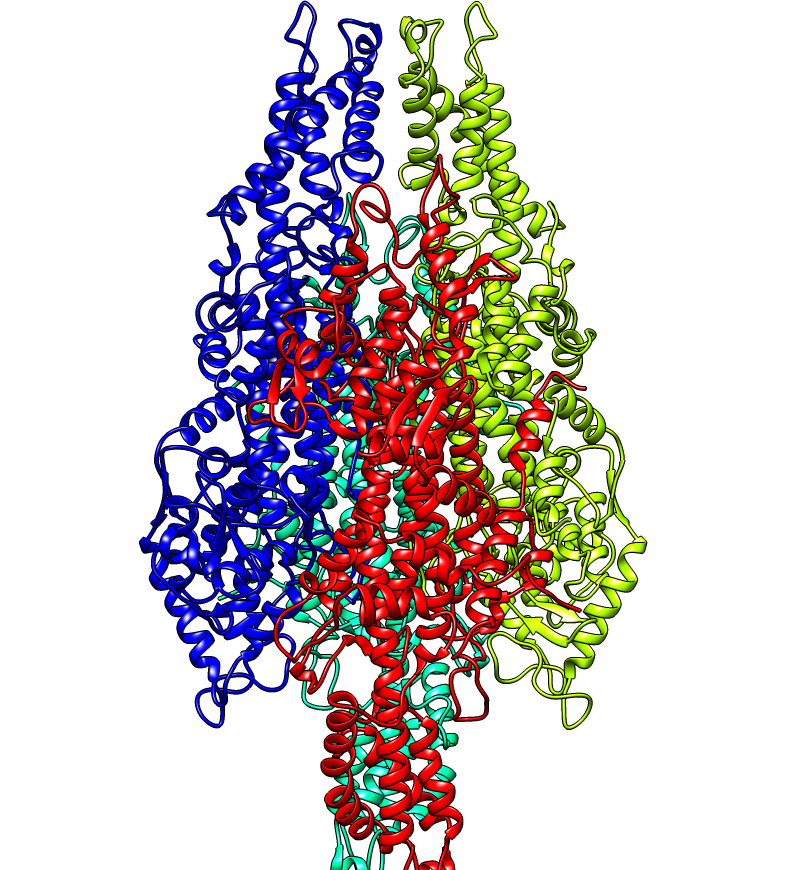
\includegraphics[width=0.5\textwidth]{../1/Minimize/model.png}
		\caption{Pn8.2617 three-dimensional model.}
		\label{fig1_1}
	\end{figure}
	\FloatBarrier
	
	\FloatBarrier
	\begin{figure}[H]
		\centering
		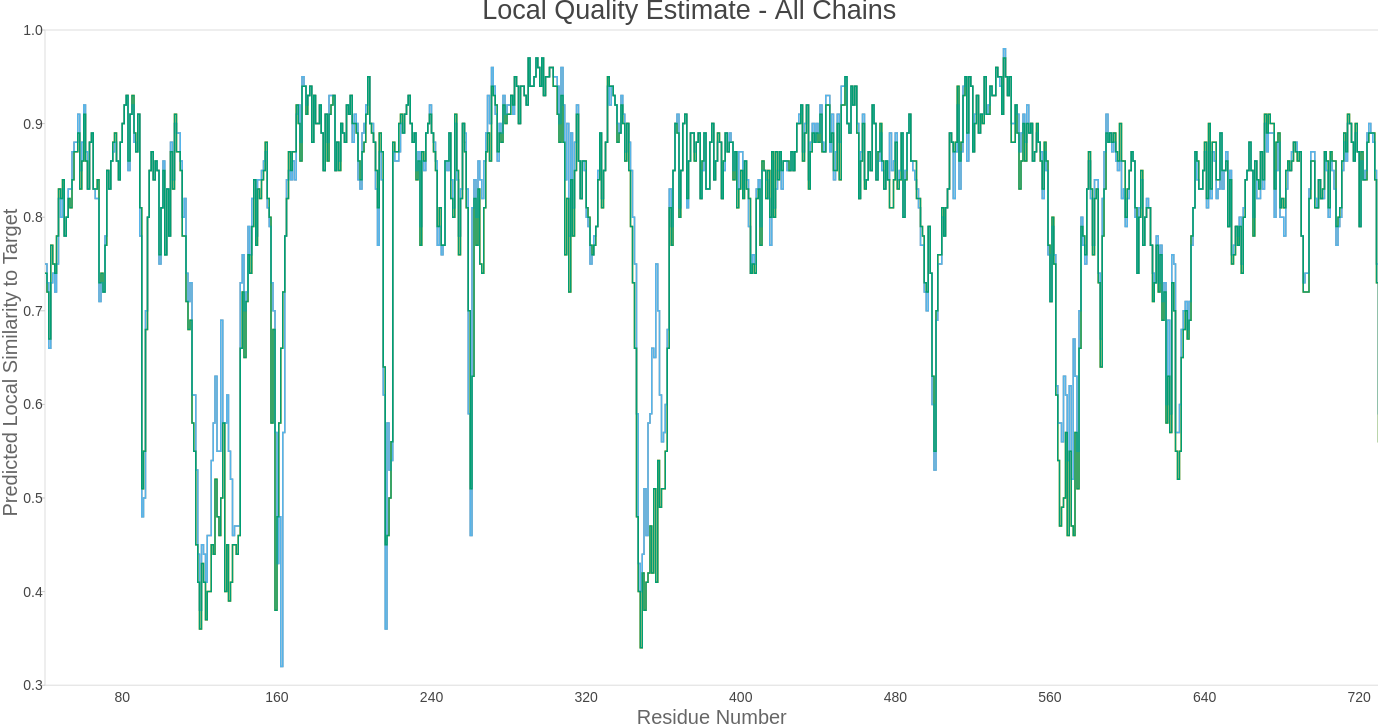
\includegraphics[width=\textwidth-50pt]{../1/Swiss/Local_quality_estimate.png}
		\caption{Pn8.2617 model QMEANDisCo.}
		\label{fig1_2}
	\end{figure}
	\FloatBarrier
	
	Before docking was performed the protein and the ligand were energy minimized. The protein structure was minimized using UCSF ChimeraX software \cite{chimera,chimera_2} and the steepest descent algorithm for 1000 steps with a step size of 0.02 \r{A}; the force field AMBER ff14SB was used for standar residues, for non standard residues the semi-empirical AM1-BCC model that uses an additive bond charge corrections was selected since it has shown higher success rate than other force fields in docking methods. \cite{am1_bcc,am1_bcc_2,am1_bcc_3}\ \ In the same way the ligand was energy minimized by using using the python library ``rdkit'' and the MMFF94 force field implemented within it. \cite{rdkit,rdkit_mmff}
	
	The preparation of the molecules for docking was made on AutoDockTools and Autodock Vina version 1.2.3 docked the protein and the ligand. \cite{adt,vina,vina_2} The grid box for the docking was selected based on the conserved domains found with the NCBI conserved domain search interface; we found the tetramer interface and active site conserved domains for phenylalanine ammonia-lyase from the CDD database. \cite{cdd,cdd_2}.  CASTp3 found the protein's pockets, which are cavities on its surface into which solvent can enter; CASTp3 uses computational geometry to find these pockets mainly using Delaunay triangulation, alpha shape, and discrete flow. \cite{castp} As a result of molecular docking with Vina, nine different conformations of the ligand in the protein were found, these results are shown in Table \ref{table1}.
	
	The docked positions of the phenylalanine in the Pn8.2617 structure interacted with different aminoacid residues of the protein (Fig. \ref{fig1_3}). Some of these aminoacids were found in the conserved domain for the active site of the enzyme, like Phe 129, Leu 147, Leu 270, Asn 274, Tyr 365, Arg 368 and Asn 398; the rest of the aminoacid that were not marked as conserved in the active site domain but were found int the pockets found by CASTp3: Phe 150, Leu 221, Phe 414, Lys 470, Glu 498, Asn 501 and Gln 502.
	
	\begin{table}[h]
		\centering
		\caption{Docking results of phenylalanine in Pn8.2617}
		\label{table1}
		\begin{tabular}{cccc}
			\toprule
			\multirow{2}{*}{Mode} & Affinity & \multicolumn{2}{c}{Dist. from best mode}\\
			&  (kcal/mol) & RMSD l.b & RMSD u.b\\
			\midrule
			1 & -6.278   &     0.0   &     0.0\\
			2 & -6.126   &   2.278   &   2.795\\
			3 & -6.098   &   1.934   &   2.262\\
			4 & -6.095   &   1.773   &   1.908\\
			5 & -6.013   &   1.735   &   2.332\\
			6 & -5.850   &   2.656   &   3.643\\
			7 & -5.847   &   1.749   &   2.333\\
			8 & -5.700   &   2.823   &   3.134\\
			9 & -5.670   &   3.526   &   4.412\\
			\bottomrule
			
		\end{tabular}
	\end{table}

	A further analysis was carried out to elucidate the protein-ligand interactions of the best conformation obtained, which has a binding energy of -6.278 kcal/mol. A search for hydrogen bonds was performed using UCSF ChimeraX allowing relax constraints of 0.4 \r{A} and 20 degrees, the bonds are shown as pseudobonds since they represent significant interactions between atoms other than covalent bonds, also because of the relax constraint these predictions can represent bonds within the tolerance values but not meeting the precise criteria. \cite{chimera,chimera_2,hbond} Four pseudobonds were found between the ligand and two aminoacid of the protein, one pseudobond with Asn 501 and a distance of 2.022 \r{A} and three with Arg 368 with distances of 2.240 \r{A}, 2.322 \r{A} and 2.438 \r{A}. In Fig. \ref{fig1_4} this pseudobonds and the ligand in its pocket are shown, the surface of the protein is colored based on its hydrophobicity using Kyte-Doolittle scale from lower (blue) to higher hydrophobicity (red).


	\FloatBarrier
	\begin{figure}[H]
		\centering
		\begin{subfigure}[H]{0.35\textwidth}
			\hspace{2cm}
			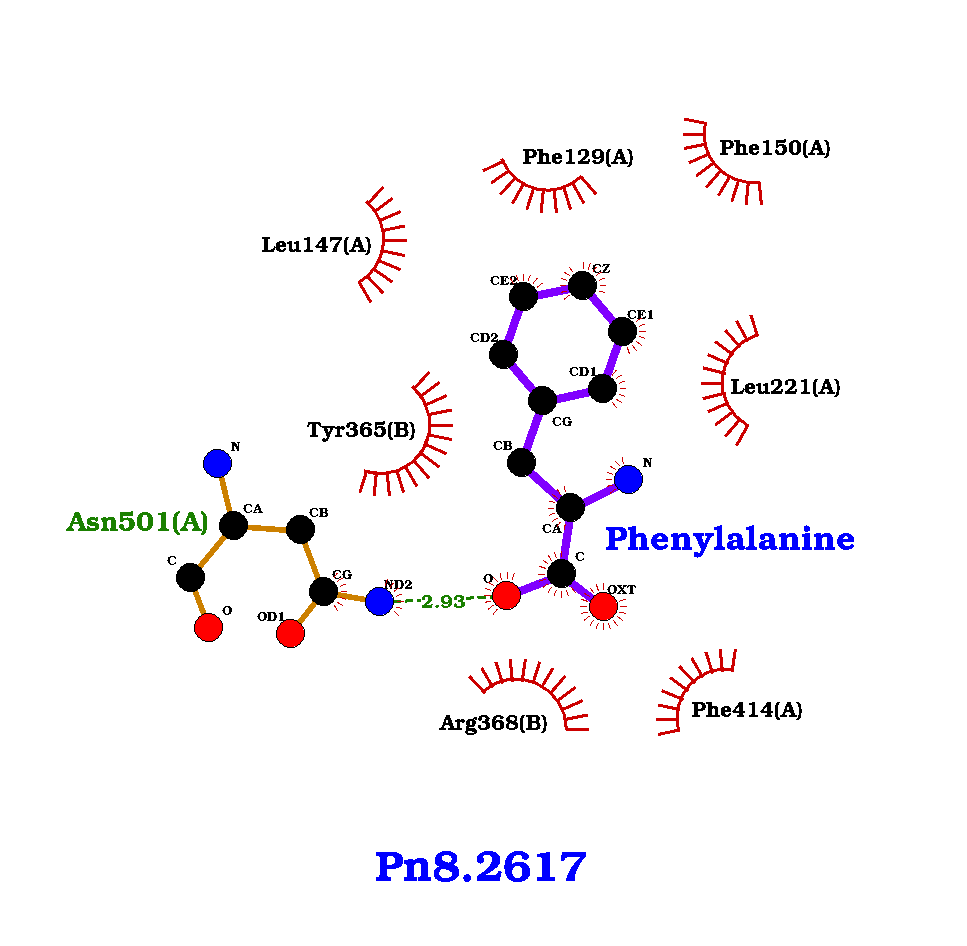
\includegraphics[width=\textwidth]{../1/Dock/best.png}
			\caption{}
		\end{subfigure}
		\hfill
		\begin{subfigure}[H]{0.35\textwidth}
			\hspace{-2cm}
			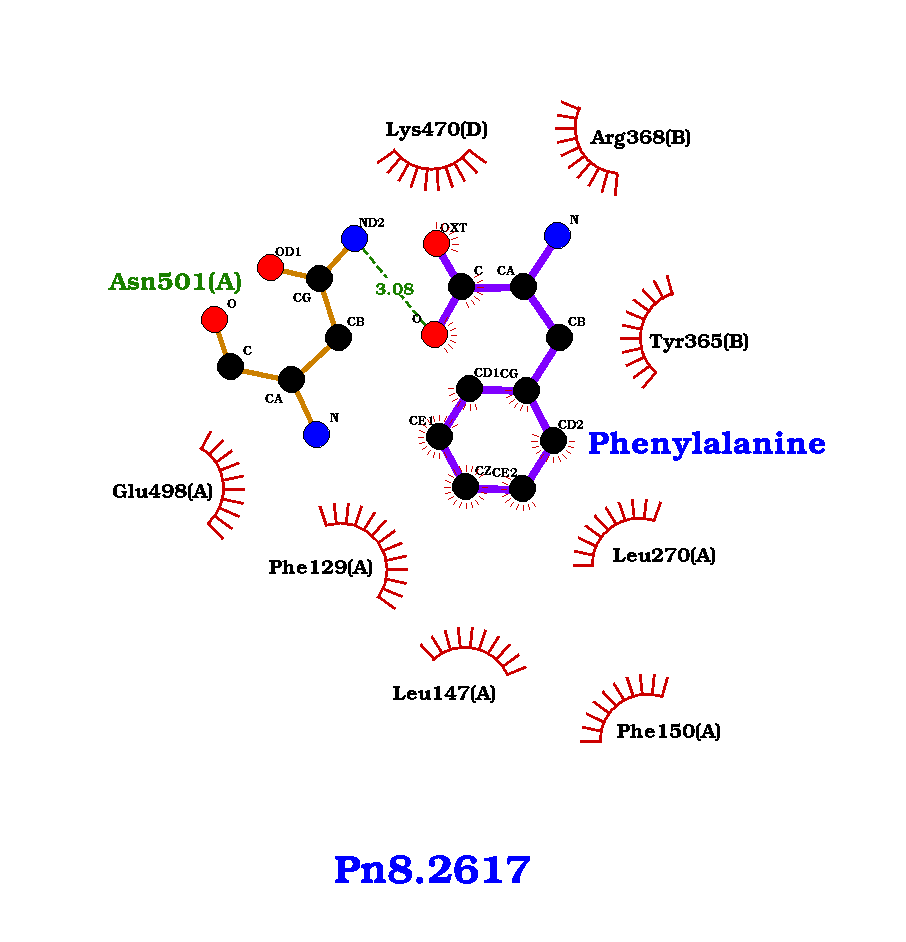
\includegraphics[width=\textwidth]{../1/Dock/best2.png}
			\caption{}
		\end{subfigure}
		\hfill
		\begin{subfigure}[H]{0.35\textwidth}
			\hspace{2cm}
			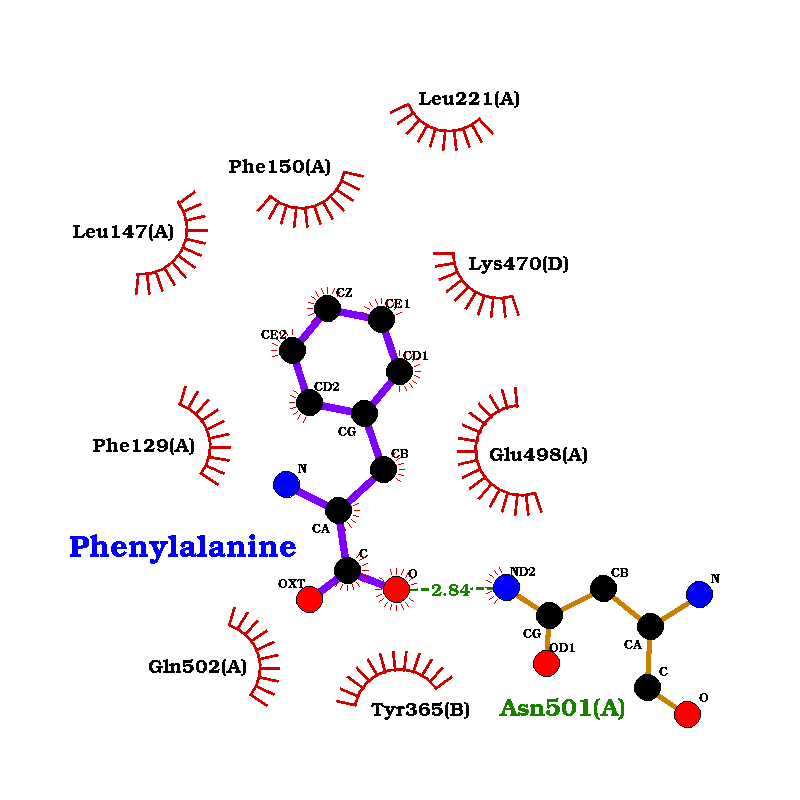
\includegraphics[width=\textwidth]{../1/Dock/best3.png}
			\caption{}
		\end{subfigure}
		\hfill
		\begin{subfigure}[H]{0.35\textwidth}
			\hspace{-2cm}
			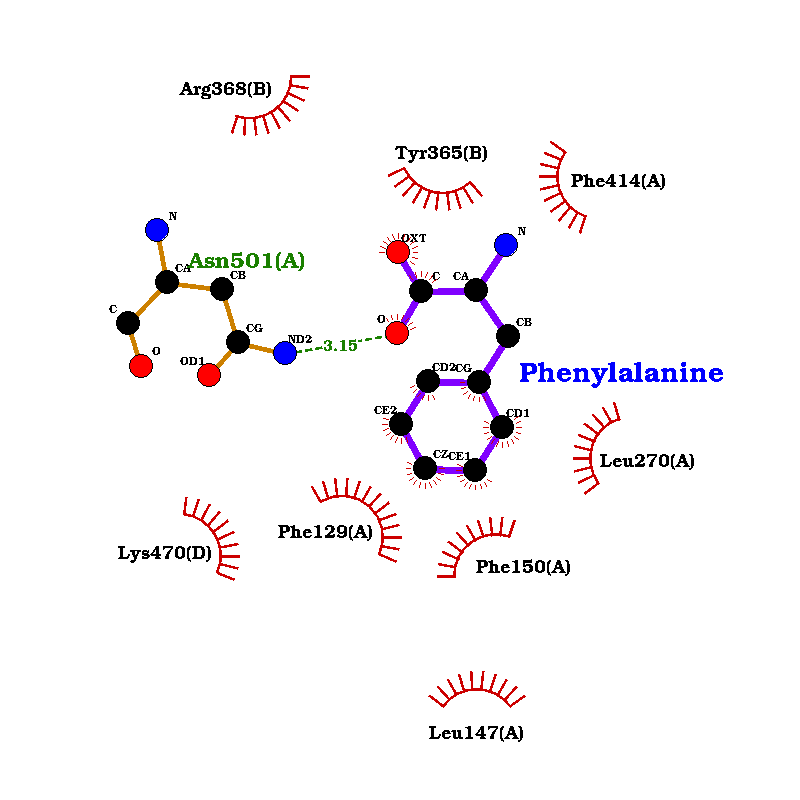
\includegraphics[width=\textwidth]{../1/Dock/best4.png}
			\caption{}
		\end{subfigure}
		\hfill
		\caption[Interactions of phenylalanine with Pn8.2617]{Interactions of phenylalanine with Pn8.2617. Best four poses are shown in order a-d.}
		\label{fig1_3}
	\end{figure}
	\FloatBarrier
	
	\FloatBarrier
	\begin{figure}[H]
		\centering
		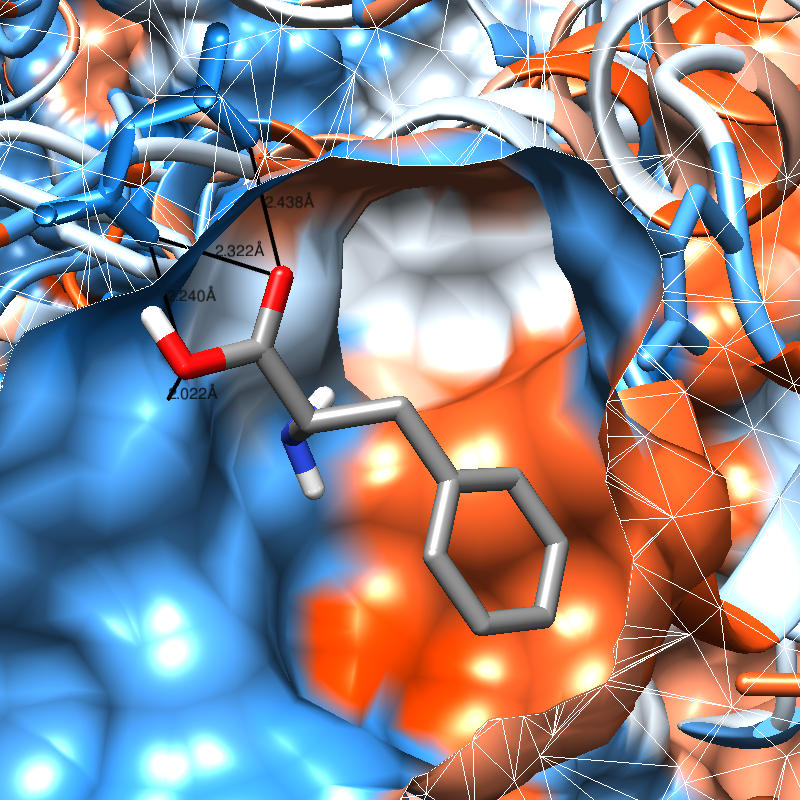
\includegraphics[width=0.4\textwidth]{../1/Dock/chimera.png}
		\caption{Phenylalanine pseudobonds with Pn8.2617.}
		\label{fig1_4}
	\end{figure}
	\FloatBarrier
	
	
	\newpage
	
	\bibliographystyle{apalike}
	\bibliography{references.bib}
	
	\newpage
	\tableofcontents
	\listoffigures
	\listoftables
	
\end{document}